% LAPA presenter deck. CS 2883R, Wed 18 Nov 2026. Juntang Wang and Vivian Hui.
% Numbers checked against arXiv 2410.11758v2; each frame comment names its source.
% Rules: one claim per frame, at most 3 bullets, no bullet restating its own figure;
% teal marks LAPA or the one number to carry; label-free IN PRETRAINING only, stage 3
% uses 100 to 7k labelled demos; equations and the setup table live in the backup.
% 15:00 for two speakers, about 14:15 budgeted. Handoff after stage 3.
% If long, cut "Policy plus decoder" first. Build: latexmk -pdf main.tex
\documentclass[aspectratio=169,12pt]{beamer}
\usetheme[progressbar=none, numbering=counter]{moloch}

\usepackage[sfdefault,light]{FiraSans}
\usepackage[T1]{fontenc}
\usepackage{tikz}
\usepackage{booktabs}
\usepackage{multicol}
\usepackage[authoryear, round]{natbib}
\definecolor{cite}{HTML}{1F5FBF}  % citations and URLs: blue, clickable
\hypersetup{colorlinks=true, citecolor=cite, urlcolor=cite, linkcolor=.}
\renewcommand{\bibsection}{}                          % the frame title is enough
\bibliographystyle{plainnat}
% Beamer 3.77 + current hyperref leave natbib's \hyper@natlinkbreak empty, which drops the
% ", " in (Author et al., 2024) and the " (" in Author et al. (2024). Restore hyperref's definition.
\makeatletter
\AddToHook{begindocument/end}{%
  \def\hyper@natlinkbreak#1#2{\hyper@linkend#1\hyper@linkstart{cite}{cite.#2}}}
\makeatother

\definecolor{ink}{HTML}{222222}
\definecolor{mute}{HTML}{8a8a8a}
\definecolor{lapa}{HTML}{12807A}     % LAPA rows and accents
\definecolor{crimson}{HTML}{A51C30}  % Harvard; title slide only

\setbeamercolor{normal text}{fg=ink, bg=white}
\setbeamercolor{frametitle}{fg=ink, bg=white}
\setbeamercolor{page number in head/foot}{fg=mute}
\setbeamertemplate{itemize items}{\color{lapa}--}
\setlength{\leftmargini}{1.1em}

\newcommand{\src}[1]{{\scriptsize\color{mute}\citep{#1}}}
\newcommand{\tbd}[3]{%
  \tikz\node[draw=lapa!60, dashed, minimum width=#1-0.4pt, minimum height=#2,
    text width=#1-6mm, align=left, font=\scriptsize, text=mute,
    execute at begin node={\hyphenpenalty=10000}]{#3};}
\newcommand{\paperfig}[3]{%
  \begin{tikzpicture}[baseline=(f.south)]
    \node[inner sep=0pt] (f) {\includegraphics[#1]{#2}};
    \node[anchor=north east, inner sep=1pt, font=\tiny, text=mute] at (f.south east)
      {\citet{ye2025lapa}, #3};
  \end{tikzpicture}}
\newcommand{\credit}[1]{\par\hfill{\tiny\color{mute}\citet{ye2025lapa}, #1}\par}
\newcommand{\lapa}[1]{{\color{lapa}#1}}
\newcommand{\colhead}[2]{\begin{minipage}[t][1.5cm]{\linewidth}\raggedright
  {\small\bfseries #1}\\\src{#2}\end{minipage}\\}
\newcommand{\s}[1]{{\tiny\color{mute}$\pm#1$}}       % std. err.
\newenvironment{notes}[1][\linewidth]
  {\begin{minipage}{#1}\footnotesize\begin{itemize}\setlength{\itemsep}{2pt}}
  {\end{itemize}\end{minipage}}

\begin{document}

% 0. Title  0:15
\begin{frame}[plain]
  \vfill
  {\LARGE\bfseries Latent Action Pretraining from Videos}\\[6pt]
  {\large\color{mute} Pretraining a robot policy on video, with no action labels}\\[-4pt]
  \textcolor{crimson}{\rule{\textwidth}{0.8pt}}\\[8pt]
  Juntang Wang $\cdot$ Vivian Hui\\[2pt]
  {\small\color{crimson} Harvard CS 2883R $\cdot$ 18 Nov 2026}\\[10pt]
  {\scriptsize\color{mute} Seonghyeon Ye, Joel Jang, et al.: KAIST, UW, Microsoft Research, NVIDIA, AI2.\\
    Latent Action Pretraining from Videos. ICLR 2025. arXiv 2410.11758}
  \vfill
\end{frame}

%% ---- Part A: problem and method, about 6:45 ----

% 1. Problem  1:00  (S1, S4.2; 970k from Kim et al. 2024 via S4.1)
\begin{frame}{Problem}
  \centering
  \paperfig{width=0.86\linewidth}{figs/fig1_problem.pdf}{Fig.~1}
  \vfill
  \begin{notes}[0.86\linewidth]
    \item A \textbf{VLA} maps an image and an instruction to a robot action
      \src{brohan2023rt2, kim2024openvla}
    \item Its training data is teleoperated: OpenVLA was pretrained on 970k demos,
      recorded one at a time
    \item \lapa{Web video is free and endless. Can it do the pretraining instead, with no
      action labels?}
  \end{notes}
  \vfill
\end{frame}

% 2. Before LAPA  0:45  (S2, S4.3)
\begin{frame}{Before LAPA}
  \begin{columns}[t]
    \column{0.31\textwidth}
      \colhead{VPT}{baker2022vpt}
      \footnotesize
      \begin{itemize}
        \item Train an inverse dynamics model on labelled data, then let it label the video
        \item Still needs labels, in the target robot's action space
      \end{itemize}
    \column{0.31\textwidth}
      \colhead{UniPi}{du2023unipi}
      \footnotesize
      \begin{itemize}
        \item Generate the future frames, then read actions off them
        \item No labels to pretrain, but the generated plans fail on long tasks
      \end{itemize}
    \column{0.31\textwidth}
      \colhead{Latent actions}{bruce2024genie, schmidt2024lapo}
      \footnotesize
      \begin{itemize}
        \item Genie and LAPO learn actions from frames alone, in games
        \item \lapa{LAPA takes this to real video and a 7B model}
      \end{itemize}
  \end{columns}
\end{frame}

% 3. Method  1:00  (S1, S3)
\begin{frame}{Method}
  \centering
  \paperfig{width=\linewidth}{figs/fig2_overview.pdf}{Fig.~2}
  \vfill
  \begin{notes}
    \item Learn a vocabulary of visual changes, learn when to use each one,
      then translate it into robot commands
    \item \lapa{Stages 1 and 2 see the same unlabelled video. Only stage 3 sees a
      robot action.}
  \end{notes}
\end{frame}

% 4. Stage 1  1:30  (S3.1; 8^4 from S4.6; H from App. F; equations in backup)
\begin{frame}{Stage 1: a vocabulary of visual changes}
  \begin{columns}[c]
    \column{0.36\textwidth}
      \centering
      \paperfig{height=4.7cm}{figs/fig8_laq.pdf}{Fig.~8}
    \column{0.62\textwidth}
      \small
      \begin{align*}
        d_1 = e_2 - e_1, \qquad
        z_1 &= \arg\min_{z_k \in C} \lVert d_1 - z_k \rVert_2 \\[2pt]
        \mathcal L &= \lVert x_2 - D(x_1, z_1) \rVert_2^2
      \end{align*}
      {\scriptsize\color{mute} $e_i$: frame embedding\, $\cdot$\, $C$: codebook\,
        $\cdot$\, $D$: decoder\, $\cdot$\, full objective in the backup\par}
      \vspace{2pt}
      \footnotesize
      \begin{itemize}\setlength{\itemsep}{2pt}
        \item The code is the \emph{difference} between two frames $0.6$\,s apart, snapped
          to the nearest of 4{,}096 entries
        \item The decoder is given $x_1$ already, so the only thing left for the code to
          carry is what changed
        \item \lapa{Encoder reads as an inverse dynamics model, decoder as a world model}
      \end{itemize}
  \end{columns}
\end{frame}

% 5. What a code looks like  1:00  (Fig. 6, S5.2) -- deliberately ahead of stage 2
\begin{frame}{What a code looks like}
  \centering
  \paperfig{width=0.76\linewidth}{figs/fig6_latent_openx.pdf}{Fig.~6}
  \vfill
  \begin{notes}[0.76\linewidth]
    \item Each column is one code, decoded into two different scenes and robot bodies
    \item \lapa{The same code gives the same coarse motion in both rows, so the vocabulary
      is shared across bodies}
    \item Nothing forces this: in human video, some codes turn out to be camera motion
      (backup)
  \end{notes}
  \vfill
\end{frame}

% 6. Stages 2 and 3  1:15  (S3.2, S3.3, fn. 2; Fig. 2 crops, trim in PDF points)
\begin{frame}{Stages 2 and 3: pretrain on codes, fine-tune to actions}
  \begin{columns}[t]
    \column{0.48\textwidth}
      \centering
      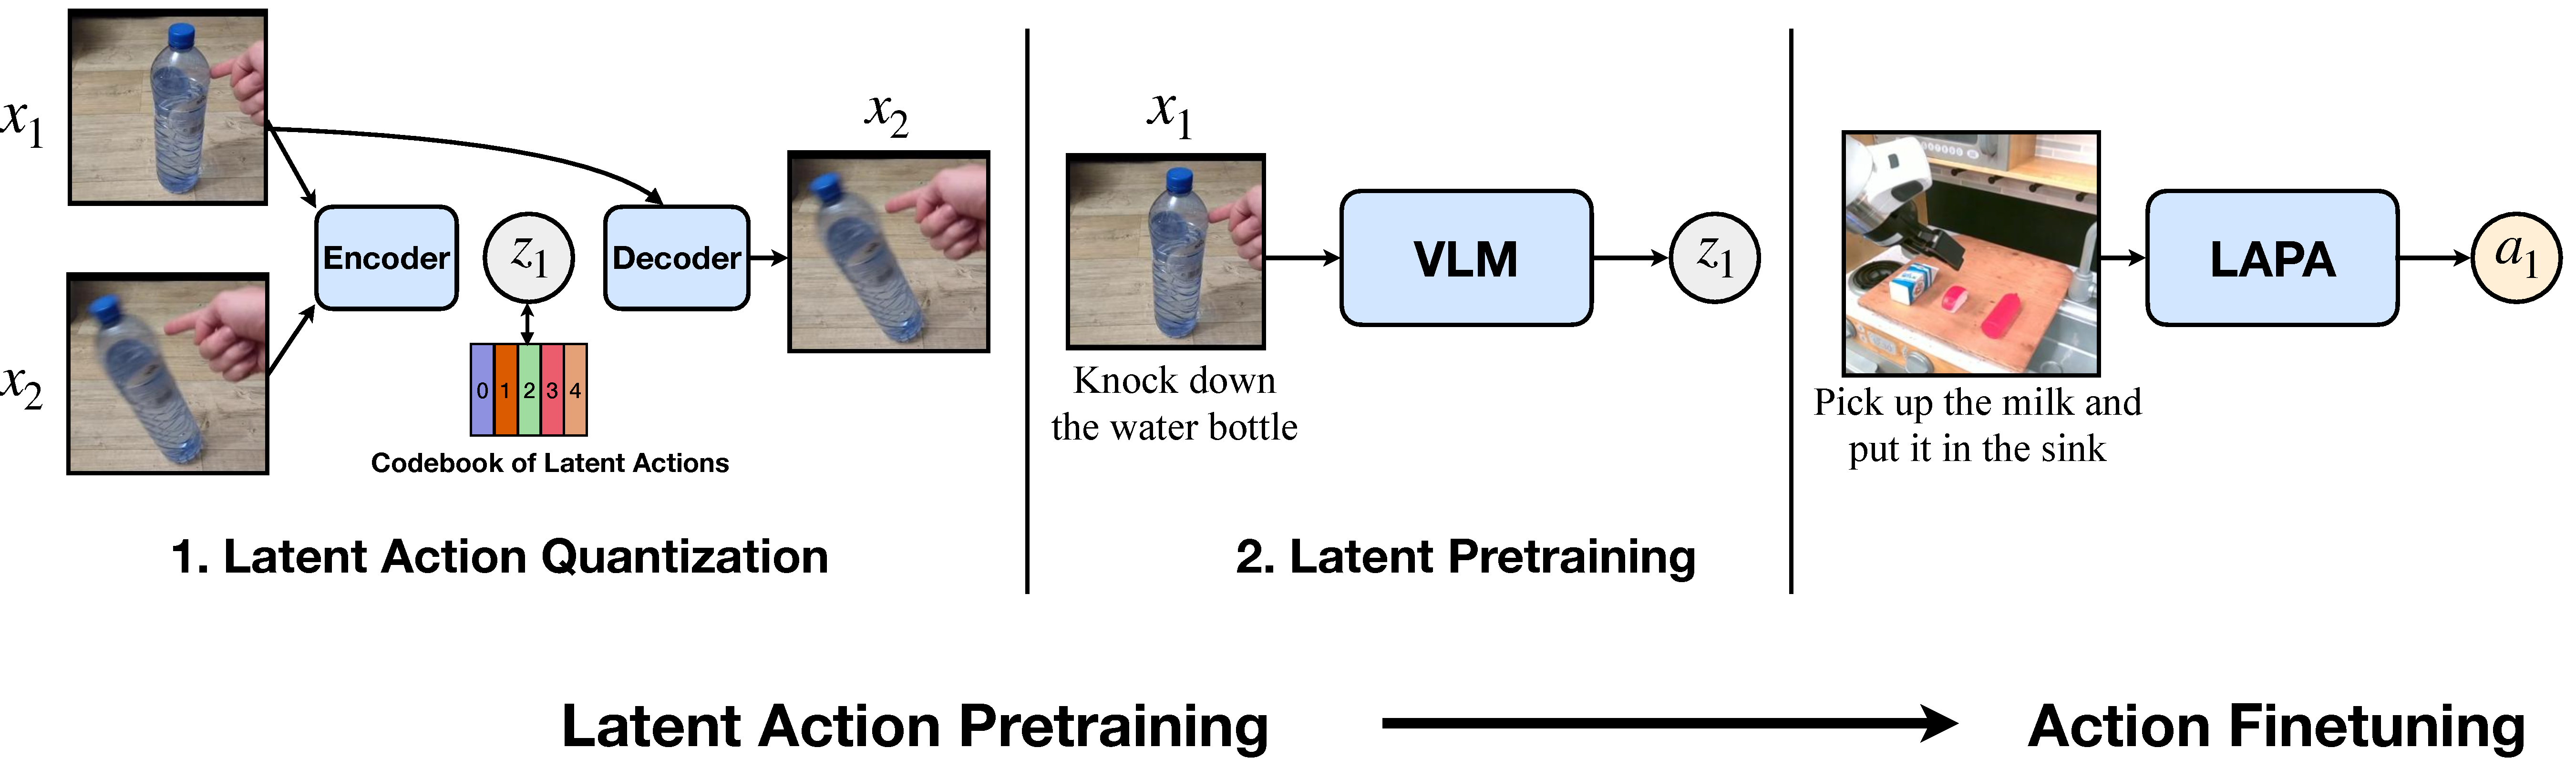
\includegraphics[height=2.3cm, trim=1050 262 804 0, clip]{figs/fig2_overview.pdf}\\[4pt]
      {\small\bfseries 2. Latent pretraining}
      \footnotesize
      \begin{itemize}\setlength{\itemsep}{3pt}
        \item Image $+$ instruction $\rightarrow$ code, supervised by stage 1's encoder
        \item A 7B video-language model \src{liu2024lwm}, a new head over the codes,
          one epoch
        \item \lapa{Any video with a language caption. No robot.}
      \end{itemize}
    \column{0.48\textwidth}
      \centering
      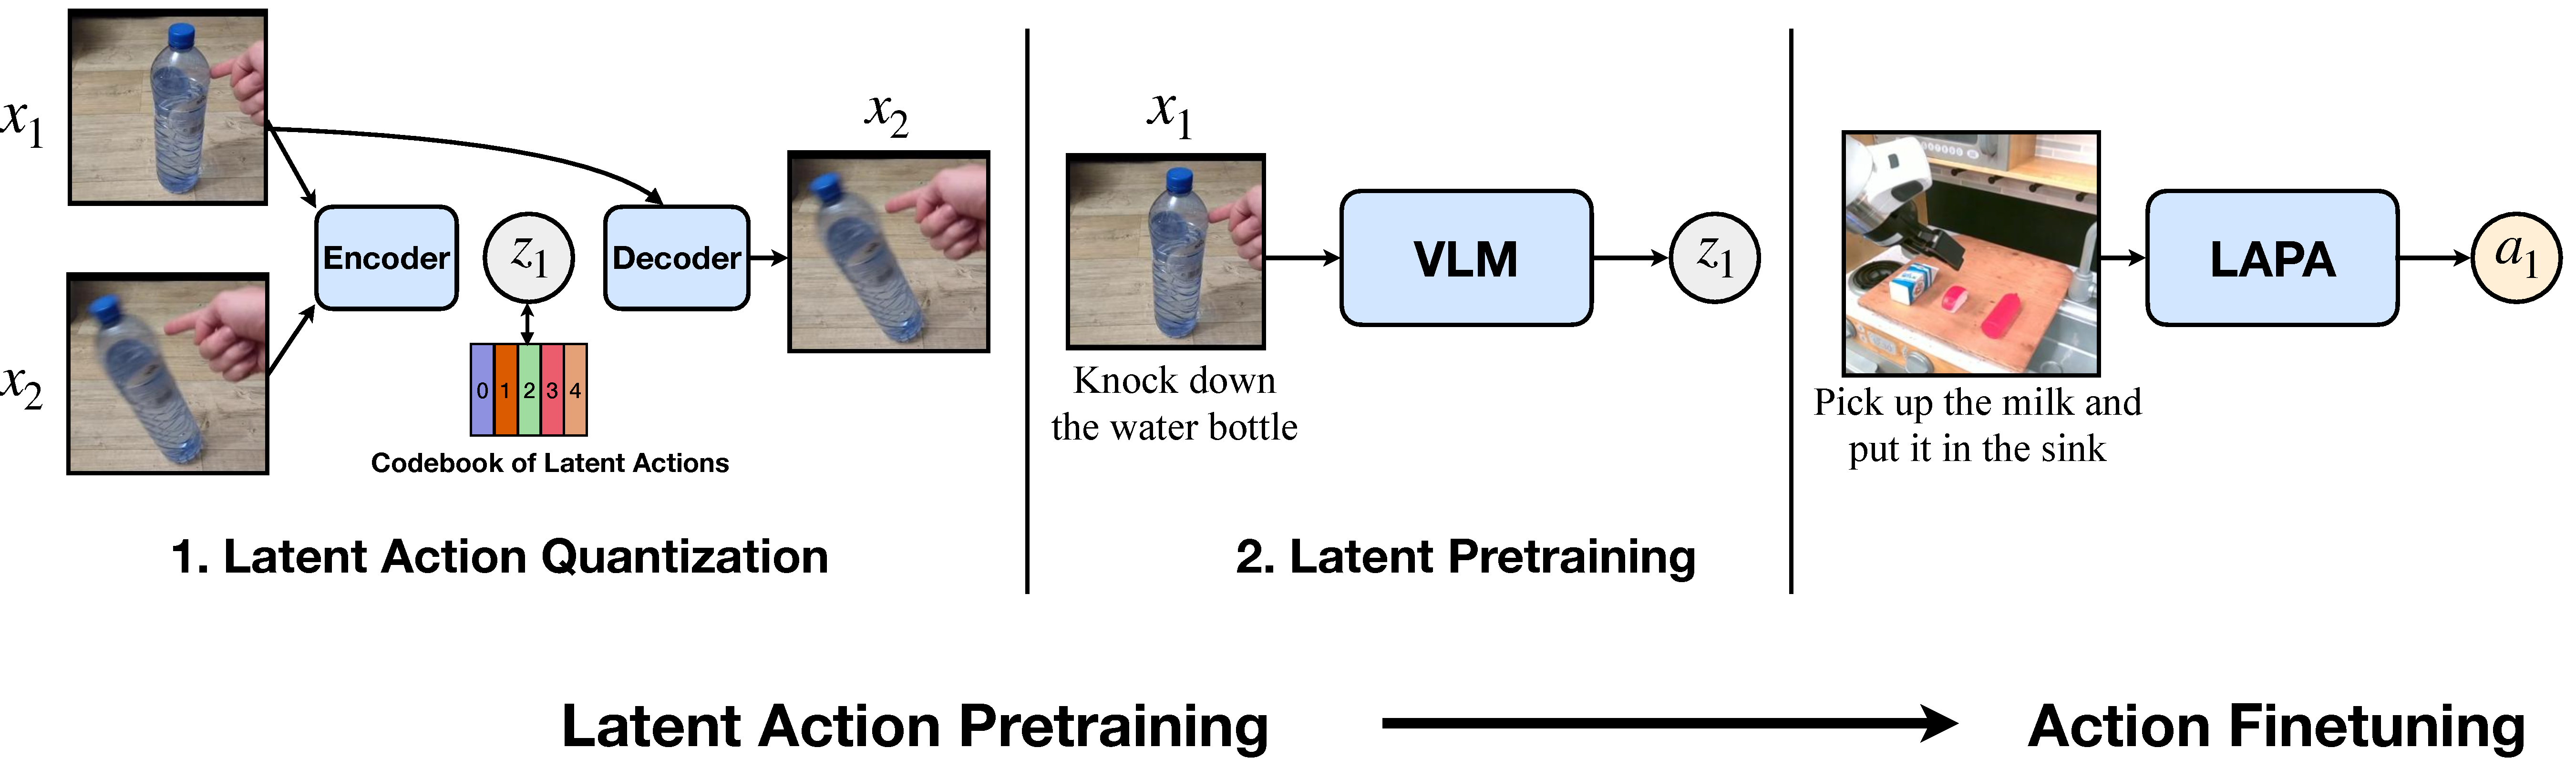
\includegraphics[height=2.3cm, trim=1815 262 0 0, clip]{figs/fig2_overview.pdf}\\[4pt]
      {\small\bfseries 3. Action fine-tuning}
      \footnotesize
      \begin{itemize}\setlength{\itemsep}{3pt}
        \item Throw the code head away; a fresh head predicts real actions
        \item Actions are small changes to the gripper: move, rotate, open or close
        \item 100 to 7k labelled demos, against OpenVLA's 970k
      \end{itemize}
  \end{columns}
  \credit{Fig.~2, middle and right}
\end{frame}

%% ==== HANDOFF: second speaker starts here (split to agree with Vivian) ====

%% ---- Part B: evidence, about 7:30 ----

% 7. Setup  0:45  (Fig. 9; full Tab. 3 in backup)
\begin{frame}{Setup}
  \centering
  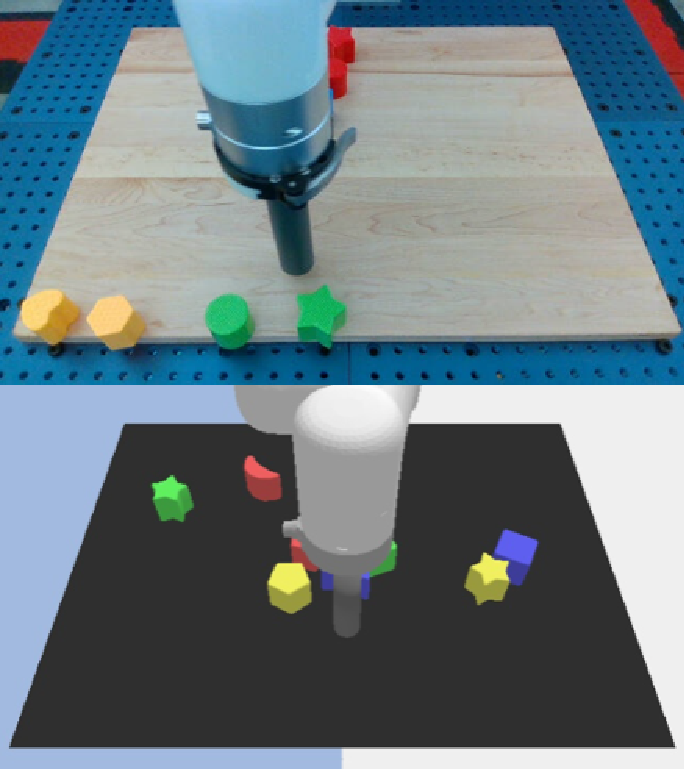
\includegraphics[height=2.3cm]{figs/fig9a_langtable.pdf}\quad
  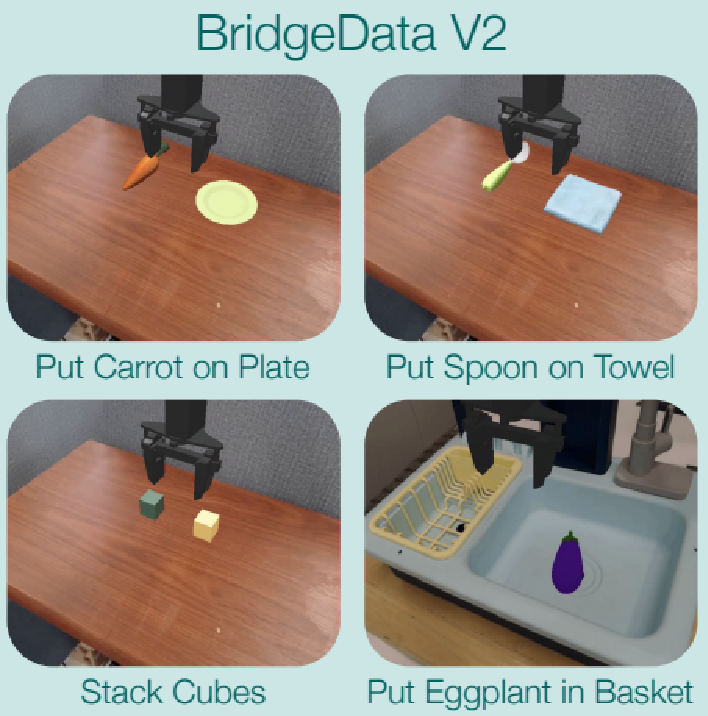
\includegraphics[height=2.3cm]{figs/fig9b_simpler.pdf}\quad
  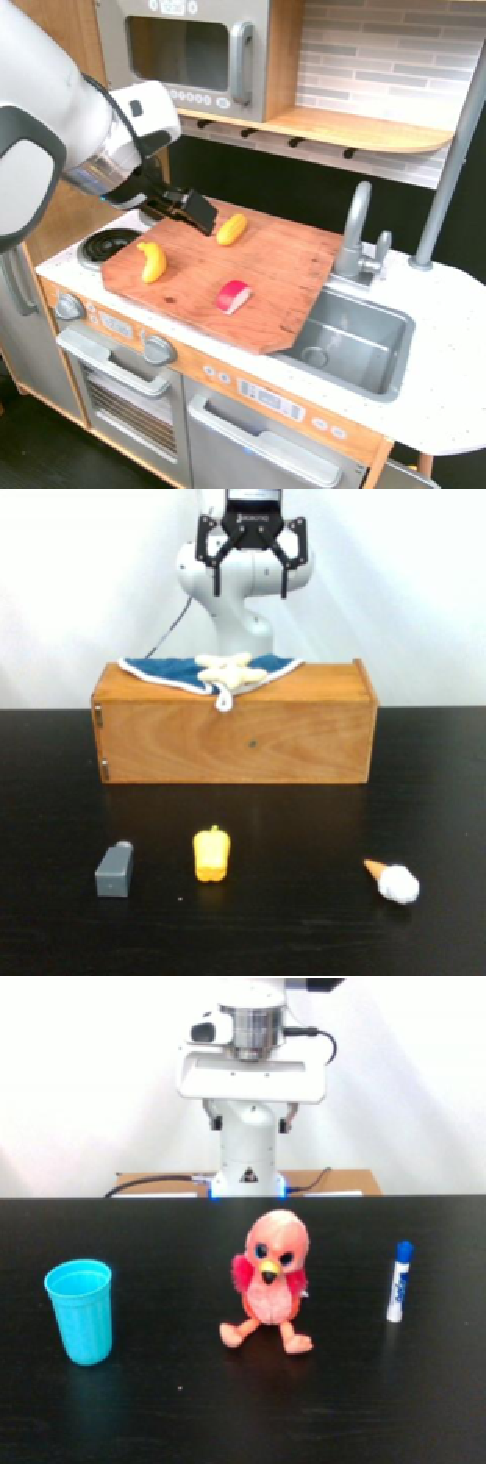
\includegraphics[height=2.3cm]{figs/fig9c_real.pdf}
  \credit{Fig.~9: Language Table and SIMPLER, both simulated, and a real Franka arm}
  \vspace{10pt}
  \begin{notes}[0.92\linewidth]
    \item Pretrain with the action labels withheld, on simulated video, Bridge (one robot),
      Open-X (many robots), or human video
    \item Fine-tune on 100 to 7k labelled demos of the test robot, then test on seen and
      unseen objects and instructions
    \item \lapa{The question each time: does pretraining without labels beat pretraining
      with them?}
  \end{notes}
  \par\vspace{10pt}
  \begin{minipage}{0.92\linewidth}\raggedright
    {\scriptsize\color{mute} Bridge \citep{walke2023bridge}, Open-X \citep{oxe2023},
      human video \citep{goyal2017something}. All eight settings in the backup.\par}
  \end{minipage}
\end{frame}

% 8. Language Table  1:00  (Tab. 1; VPT's 7k from S4.3)
\begin{frame}{Results: Language Table}
  \centering\scriptsize
  \setlength{\tabcolsep}{4pt}
  \begin{tabular}{@{}l*{6}{c}@{}}
    \toprule
    & \multicolumn{2}{c}{in-domain (1k)} & \multicolumn{2}{c}{cross-task (7k)}
      & \multicolumn{2}{c}{cross-env (1k)} \\
    \cmidrule(lr){2-3}\cmidrule(lr){4-5}\cmidrule(l){6-7}
    & seen & unseen & seen & unseen & seen & unseen \\
    \midrule
    Scratch & 15.6\s{9.2} & 15.2\s{8.3} & 27.2\s{13.6} & 22.4\s{11.0} & 15.6\s{9.2} & 15.2\s{8.3} \\
    UniPi & 22.0\s{12.5} & 13.2\s{7.7} & 20.8\s{12.0} & 16.0\s{9.1} & 13.6\s{8.6} & 12.0\s{7.5} \\
    VPT & 44.0\s{7.5} & 32.8\s{4.6} & 72.0\s{6.8} & \textbf{60.8}\s{6.6} & 18.0\s{7.7} & 18.4\s{9.7} \\
    \lapa{LAPA} & \textbf{62.0}\s{8.7} & \textbf{49.6}\s{9.5} & \textbf{73.2}\s{6.8} & 54.8\s{9.1}
      & \textbf{33.6}\s{12.7} & \textbf{29.6}\s{12.0} \\
    \midrule
    \color{mute}ActionVLA & \color{mute}77.0\s{3.5} & \color{mute}58.8\s{6.6} & \color{mute}77.0\s{3.5}
      & \color{mute}58.8\s{6.6} & \color{mute}64.8\s{5.2} & \color{mute}54.0\s{7.0} \\
    \bottomrule
  \end{tabular}
  \credit{Tab.~1: success rate (\%) $\pm$ std.\ err.; bold = best of the top four rows;
    ActionVLA pretrains on the true actions}
  \vfill
  \begin{notes}
    \item LAPA leads 5 of 6 columns. VPT wins cross-task unseen, where its labeller was
      trained on the 7k labelled demos
    \item Cross-env, pretrained on real video and tested in simulation, is where a
      label-trained labeller stops transferring and LAPA still helps
    \item The error bars overlap almost everywhere: read the ordering, not the gaps
  \end{notes}
  \vfill
\end{frame}

% 9. Real robot  1:15  (Fig. 3, Tab. 2, S4.4, App. B)
\begin{frame}{Results: real robot}
  \centering
  \paperfig{width=0.92\linewidth}{figs/fig3_real.pdf}{Fig.~3}
  \vfill
  \begin{notes}[0.92\linewidth]
    \item Franka arm, 3 tasks, 54 attempts each, partial credit for reaching and grasping
    \item Pretrained on Open-X: \lapa{LAPA 50.1} against OpenVLA's 43.9, ahead on all
      three kinds of generalization
    \item Pretrained on Bridge, LAPA also beats both action-labelled models. The authors'
      reading: labels overfit the policy to one robot's action space
  \end{notes}
  \vfill
\end{frame}

% 10. Human video only  1:00  (Fig. 4, S4.5; clip counts App. D)
\begin{frame}{Results: human video only}
  \centering
  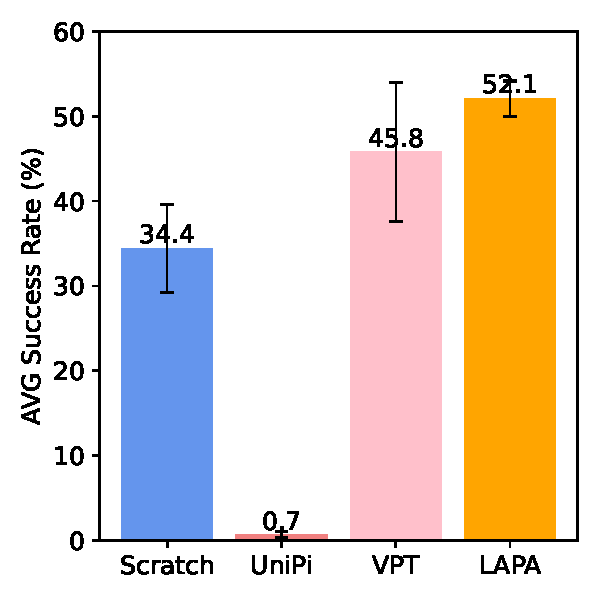
\includegraphics[height=3.4cm]{figs/fig4a_human_simpler.pdf}\hfill
  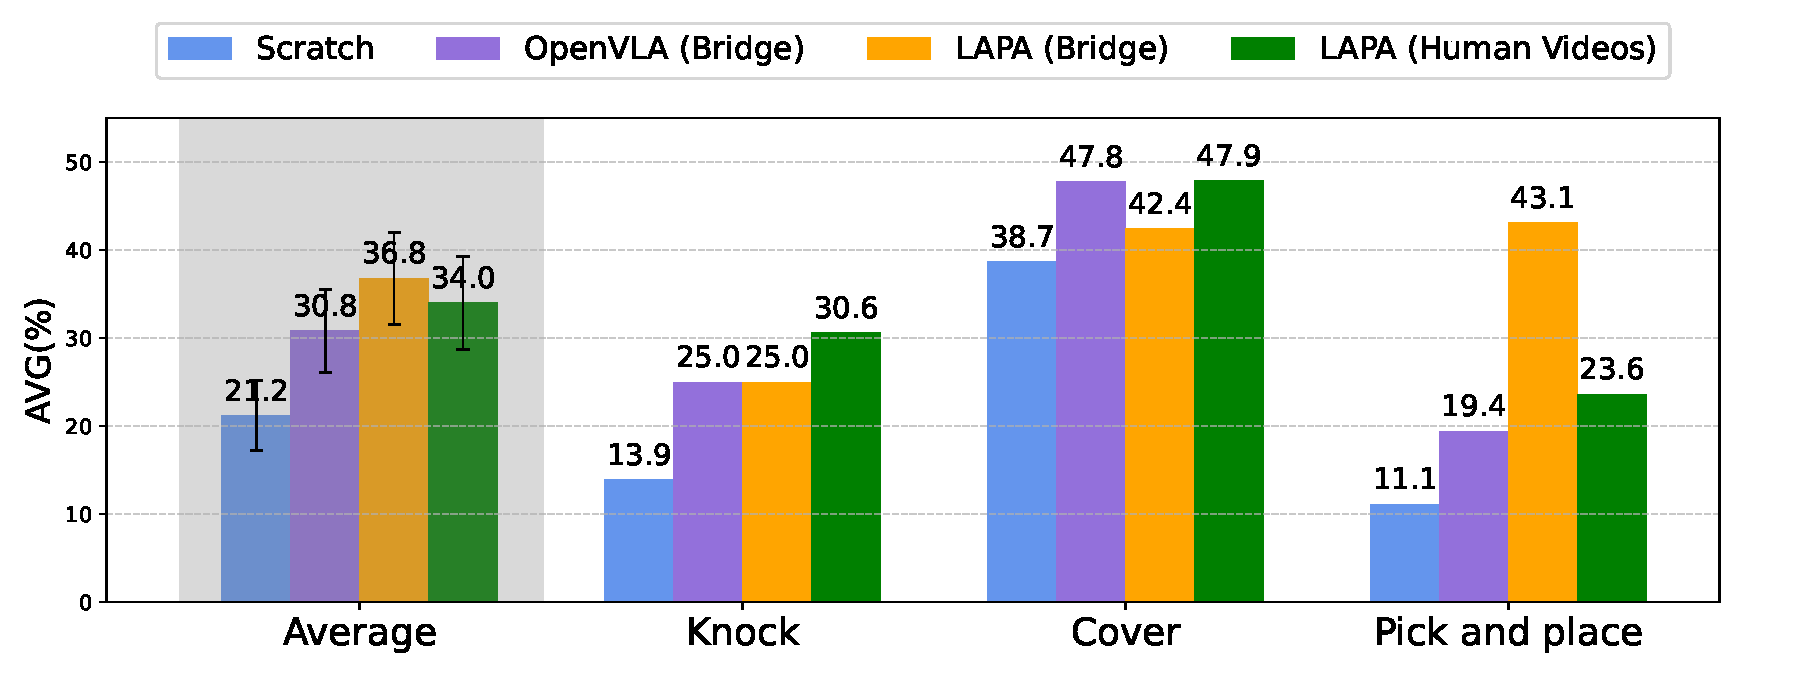
\includegraphics[height=3.4cm]{figs/fig4b_human_real.pdf}
  \credit{Fig.~4: (a) SIMPLER, (b) real robot}
  \vfill
  \begin{notes}
    \item Pretrained on Something-Something v2 alone: no robot, no actions, a 2.4\,s window
    \item Real robot \lapa{34.0}: above OpenVLA pretrained on Bridge (30.8), below OpenVLA
      pretrained on Open-X (43.9)
    \item The three test tasks suit the corpus: it holds 6{,}655 ``knocking'' clips where
      Bridge holds 2
  \end{notes}
  \vfill
\end{frame}

% 11. Pretraining cost  0:30  (S4.6, fn. 5)
\begin{frame}{Pretraining cost}
  \centering\small
  \setlength{\tabcolsep}{8pt}
  \begin{tabular}{@{}lrr@{}}
    \toprule
    & \lapa{LAPA (Open-X)} & OpenVLA \\
    \midrule
    GPU-hours & 272 H100 & 21{,}500 A100 \\
    batch size & 128 & 2048 \\
    output space per step & $8^4$ & $256^7$ \\
    \bottomrule
  \end{tabular}
  \credit{\S4.6: ``approximately 30--40 times more efficient''}
  \vfill
  \begin{notes}[0.8\linewidth]
    \item The authors attribute it to the backbone, already trained on video, and to the
      tiny output space
    \item Not an end-to-end audit: two different accelerators, and the cost of training
      stage 1 is not reported
  \end{notes}
  \vfill
\end{frame}

% 12. Policy plus decoder  0:45  (Fig. 7, S5.2) -- first to cut if running long
\begin{frame}{Policy plus decoder}
  \centering
  \paperfig{width=\linewidth}{figs/fig7_rollout.pdf}{Fig.~7}
  \vfill
  \begin{notes}
    \item A pretrained LAPA, never fine-tuned, picks codes for ``take the broccoli out of
      the pot''
    \item \lapa{Stage 1's decoder renders each next frame, and that frame becomes the next
      input: a closed loop with no robot}
    \item Eight frames, one example, no metric. Suggestive of a world model, not yet
      evidence of one
  \end{notes}
  \vfill
\end{frame}

% 13. Limitations  0:45  (S6; ours from App. B, D, E, F and fn. 1)
\begin{frame}{Limitations}
  \begin{columns}[t]
    \column{0.46\textwidth}
      {\small\bfseries Stated} {\scriptsize\color{mute}(\S6)}
      \footnotesize
      \begin{itemize}\setlength{\itemsep}{3pt}
        \item A code spans 0.6\,s, too coarse for grasping
        \item 7B inference latency, as for any VLA
        \item Manipulation only; no driving or navigation
      \end{itemize}
    \column{0.50\textwidth}
      {\small\bfseries Ours}
      \footnotesize
      \begin{itemize}\setlength{\itemsep}{3pt}
        \item The language labels are not free. All three corpora ship with text
        \item LAPA and OpenVLA tie in 51.9\% of the real-robot attempts
        \item Codes absorb camera motion, and the policy sees one frame, no history
        \item The SIMPLER fine-tuning demos came from a Bridge-trained policy
      \end{itemize}
  \end{columns}
\end{frame}

% 14. Takeaway  0:30
\begin{frame}{Takeaway}
  \vfill
  \begin{columns}
    \column{0.88\textwidth}
      \begin{itemize}\setlength{\itemsep}{10pt}
        \item LAPA replaces the action labels \emph{in pretraining} with a learned
          vocabulary of visual changes. Downstream it still needs demos, just a hundred
          or so instead of a million
        \item \lapa{Where it wins is crossing from one robot body to another, which is
          exactly where action labels turn out to hurt}
        \item What is shown is strong; what is claimed around it, a world model and
          label-free robotics, is not shown yet
      \end{itemize}
  \end{columns}
  \vfill
\end{frame}

% 15. Discussion  -- the 15 minutes end here; call on the roles
\begin{frame}{Discussion}
  \begin{columns}[t]
    \column{0.42\textwidth}
      {\small\bfseries Roles, in call order}\\[4pt]
      \tbd{\linewidth}{3.4cm}{From the Ed post and the role sheet (second tab). 5 minutes each.}
    \column{0.54\textwidth}
      {\small\bfseries Open questions}
      \footnotesize
      \begin{itemize}\setlength{\itemsep}{6pt}
        \item What can a code between two frames never capture: force, grasp timing, speed?
        \item Is the gain from the latent actions, or from a backbone already trained on
          video? Nothing in the paper swaps it out
        \item What would have to be true before a decoder rollout could stand in for a
          real-robot trial?
      \end{itemize}
  \end{columns}
\end{frame}

%% ---- backup ----
\appendix

% App. A, eqs. (1) to (4)
\begin{frame}{Backup: stage 1 objective}
  \footnotesize
  \begin{align*}
    z_1 &= \arg\min_{z_k \in C} \lVert d_1 - z_k \rVert_2,
      \quad d_1 = e_2 - e_1 \tag{1}\\
    \hat d_1 &= d_1 + \frac{\lVert d_1 - z_1 \rVert}{\lVert v \rVert}\, v,
      \quad v \sim \mathcal N(0, 1) \tag{2}\\
    \hat x_2 &= D\big(\mathrm{Attn}(\mathrm{sg}[p_1], \hat d_1, \hat d_1)\big) \tag{3}\\
    \mathcal L &= \lVert x_2 - \hat x_2 \rVert_2^2 \tag{4}
  \end{align*}
  \credit{App.~A}
  \vfill
  \begin{notes}
    \item $e_1, e_2$: C-ViViT \src{villegas2023phenaki} embeddings of $x_1$ and $x_2$;
      $p_1$: patch embedding of $x_1$; $C$: the codebook
    \item (2) is NSVQ \src{vali2022nsvq}: substitute noise of the same magnitude as the
      quantization error, so the codebook stays differentiable and codes stop dying
    \item (3) stops the gradient through $p_1$, or the encoder and decoder collude and the
      code carries nothing
  \end{notes}
\end{frame}

\begin{frame}{Backup: the eight experiments}
  \centering
  {\scriptsize
  \setlength{\tabcolsep}{8pt}
  \renewcommand{\arraystretch}{1.05}
  \begin{tabular}{@{}lllrr@{}}
    \toprule
    benchmark & test & pretrain on, no labels & trajs & fine-tune \\
    \midrule
    Language Table \src{lynch2023language} & in-domain & sim & 181k & 1k \\
      & cross-task & sim & 181k & 7k \\
      & cross-env & real & 442k & 1k \\
    SIMPLER \src{li2024simpler} & in-domain & Bridge & 60k & 100 \\
      & cross-body & human video & 200k & 100 \\
    Real Franka & cross-body & Bridge & 60k & 450 \\
      & many bodies & Open-X & 970k & 450 \\
      & cross-body & human video & 200k & 450 \\
    \bottomrule
  \end{tabular}}
  \credit{Tab.~3}
  {\tiny\color{mute} Bridge \citep{walke2023bridge}; Open-X \citep{oxe2023};
    human video: Something-Something v2 \citep{goyal2017something}.
    Tab.~3 gives 200k Something-Something videos, \S4.5 gives 220K.\par}
\end{frame}

\begin{frame}{Backup: real robot by generalization type}
  \centering\small
  \setlength{\tabcolsep}{8pt}
  \begin{tabular}{@{}lcccc@{}}
    \toprule
    & seen objects, & unseen & seen objects, & \\
    & unseen combo & objects & unseen instr. & average \\
    \midrule
    Scratch & 18.0 & 20.3 & 25.4 & 21.2 \\
    \midrule
    ActionVLA (Bridge) & 38.3 & 31.8 & 27.7 & 32.6 \\
    OpenVLA (Bridge) & 35.6 & 34.6 & 22.1 & 30.8 \\
    \lapa{LAPA (Bridge)} & 43.4 & 31.4 & 35.6 & 36.8 \\
    \midrule
    OpenVLA (Open-X) & 46.2 & 42.1 & 43.4 & 43.9 \\
    \lapa{LAPA (Open-X)} & \textbf{57.8} & \textbf{43.9} & \textbf{48.5} & \textbf{50.1} \\
    \midrule
    \lapa{LAPA (human video)} & 36.5 & 37.4 & 28.1 & 34.0 \\
    \bottomrule
  \end{tabular}
  \credit{Tab.~2: success rate (\%), partial credit, 54 attempts per model}
\end{frame}

\begin{frame}{Backup: scaling}
  \centering
  \begin{minipage}[t]{0.24\linewidth}\centering
    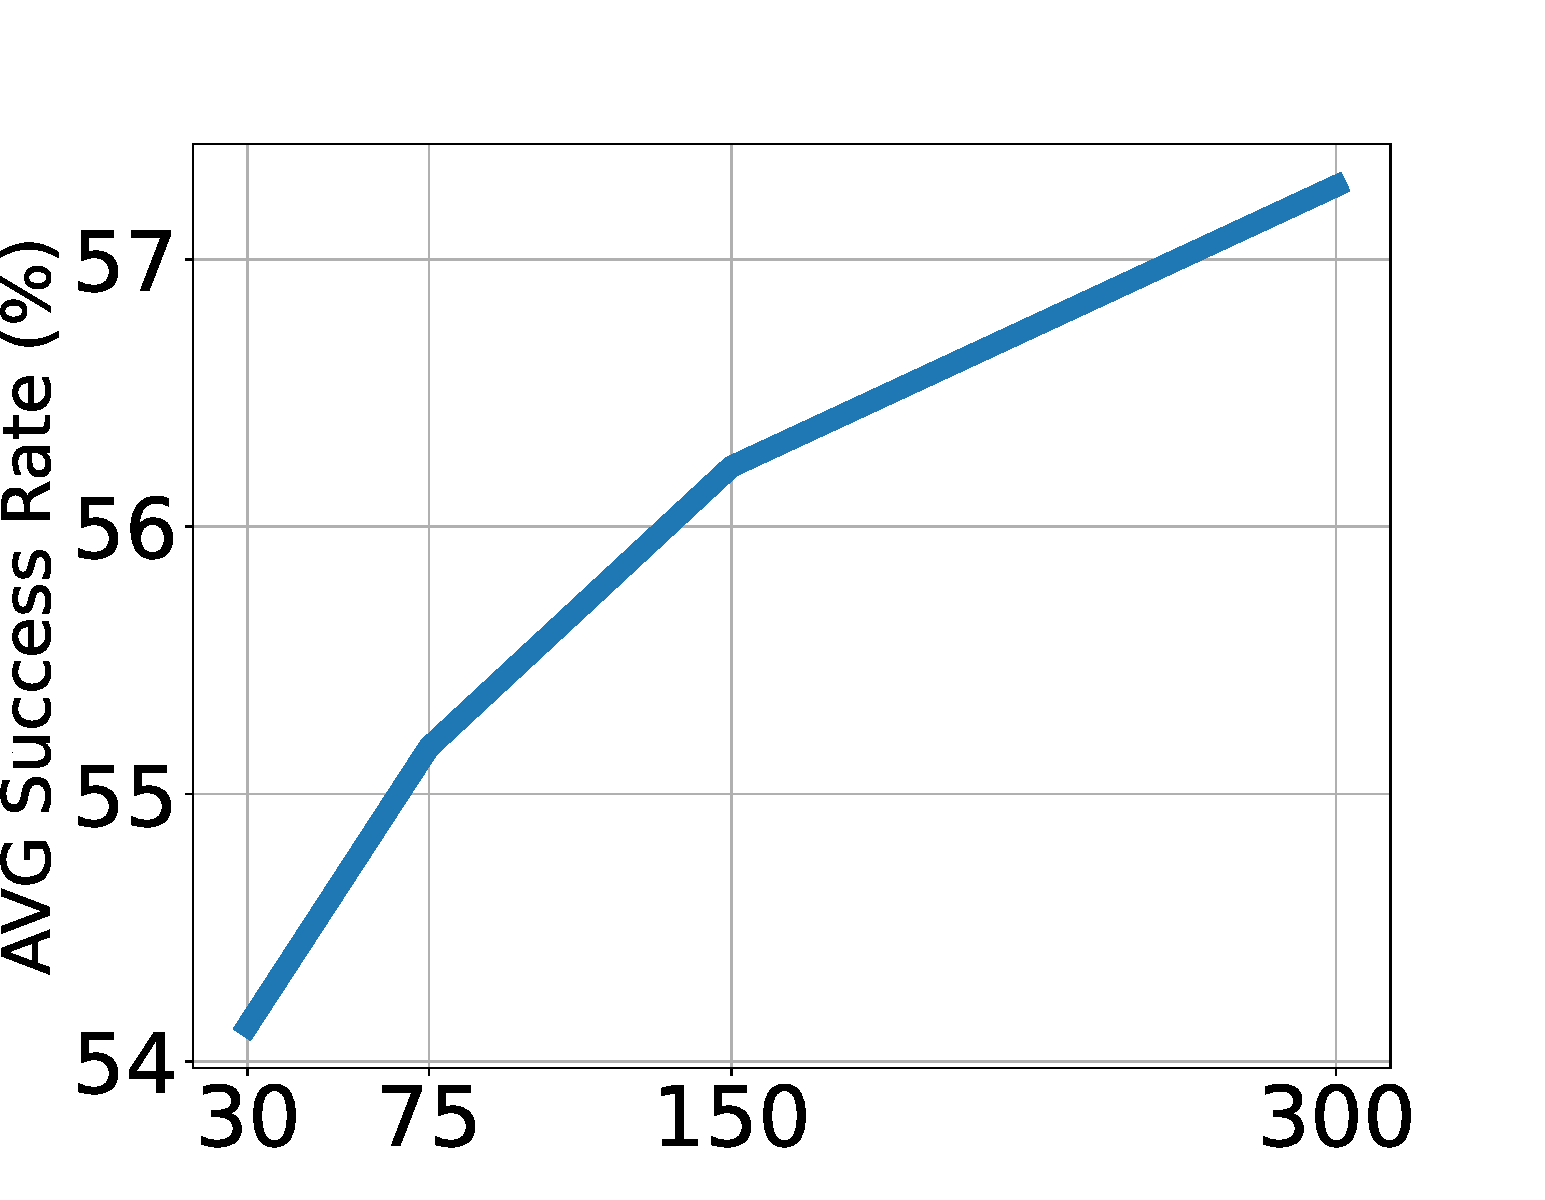
\includegraphics[width=\linewidth]{figs/fig5a_model.pdf}\\{\scriptsize model size (M)}\end{minipage}\hfill
  \begin{minipage}[t]{0.24\linewidth}\centering
    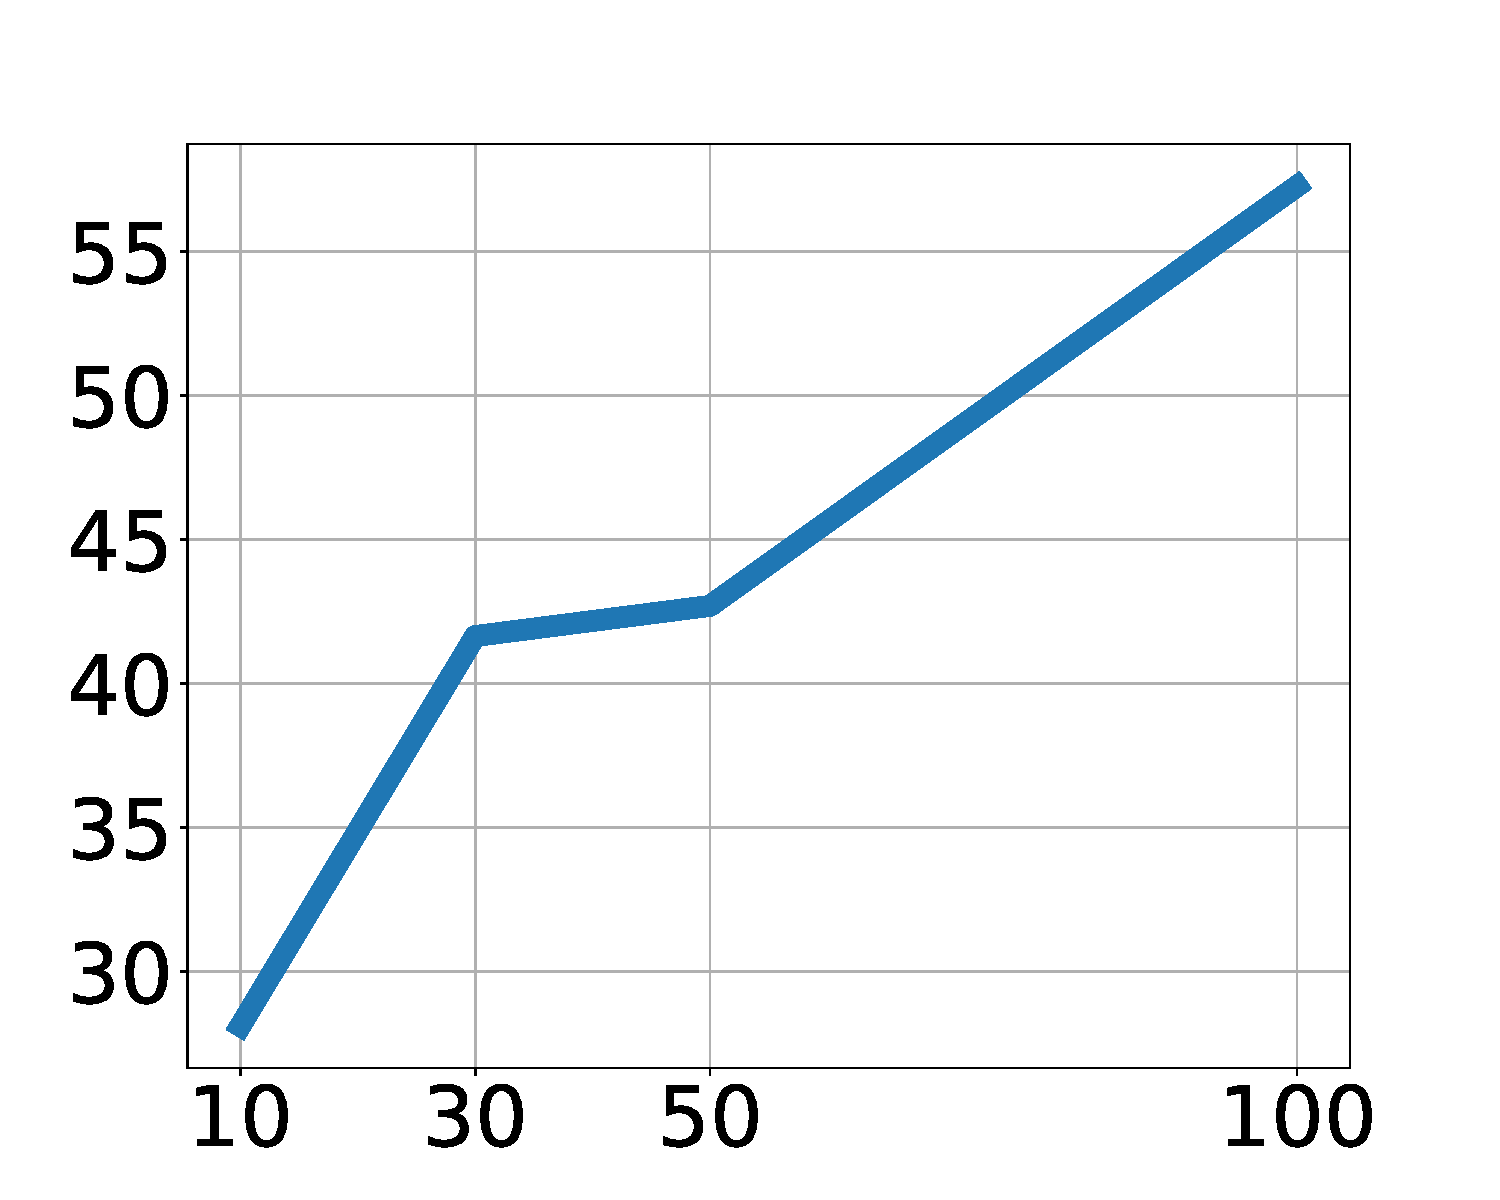
\includegraphics[width=\linewidth]{figs/fig5b_data.pdf}\\{\scriptsize data (\% of Bridge)}\end{minipage}\hfill
  \begin{minipage}[t]{0.24\linewidth}\centering
    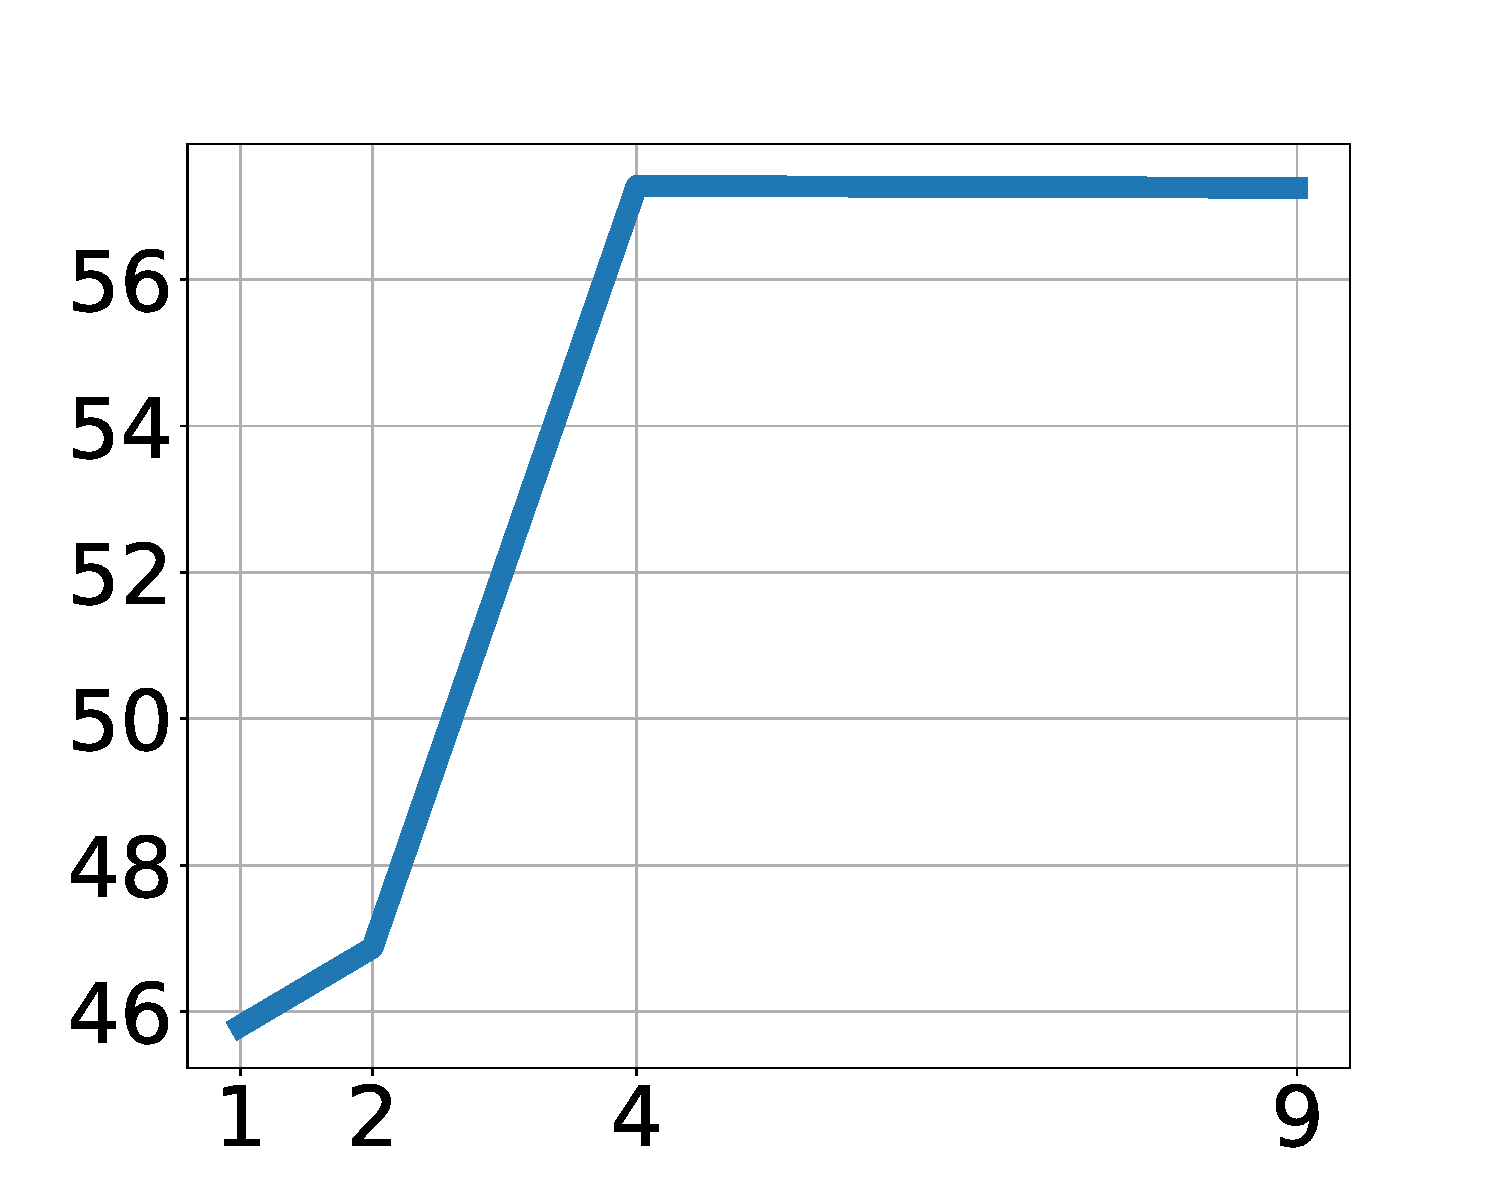
\includegraphics[width=\linewidth]{figs/fig5c_length.pdf}\\{\scriptsize latent length}\end{minipage}\hfill
  \begin{minipage}[t]{0.24\linewidth}\centering
    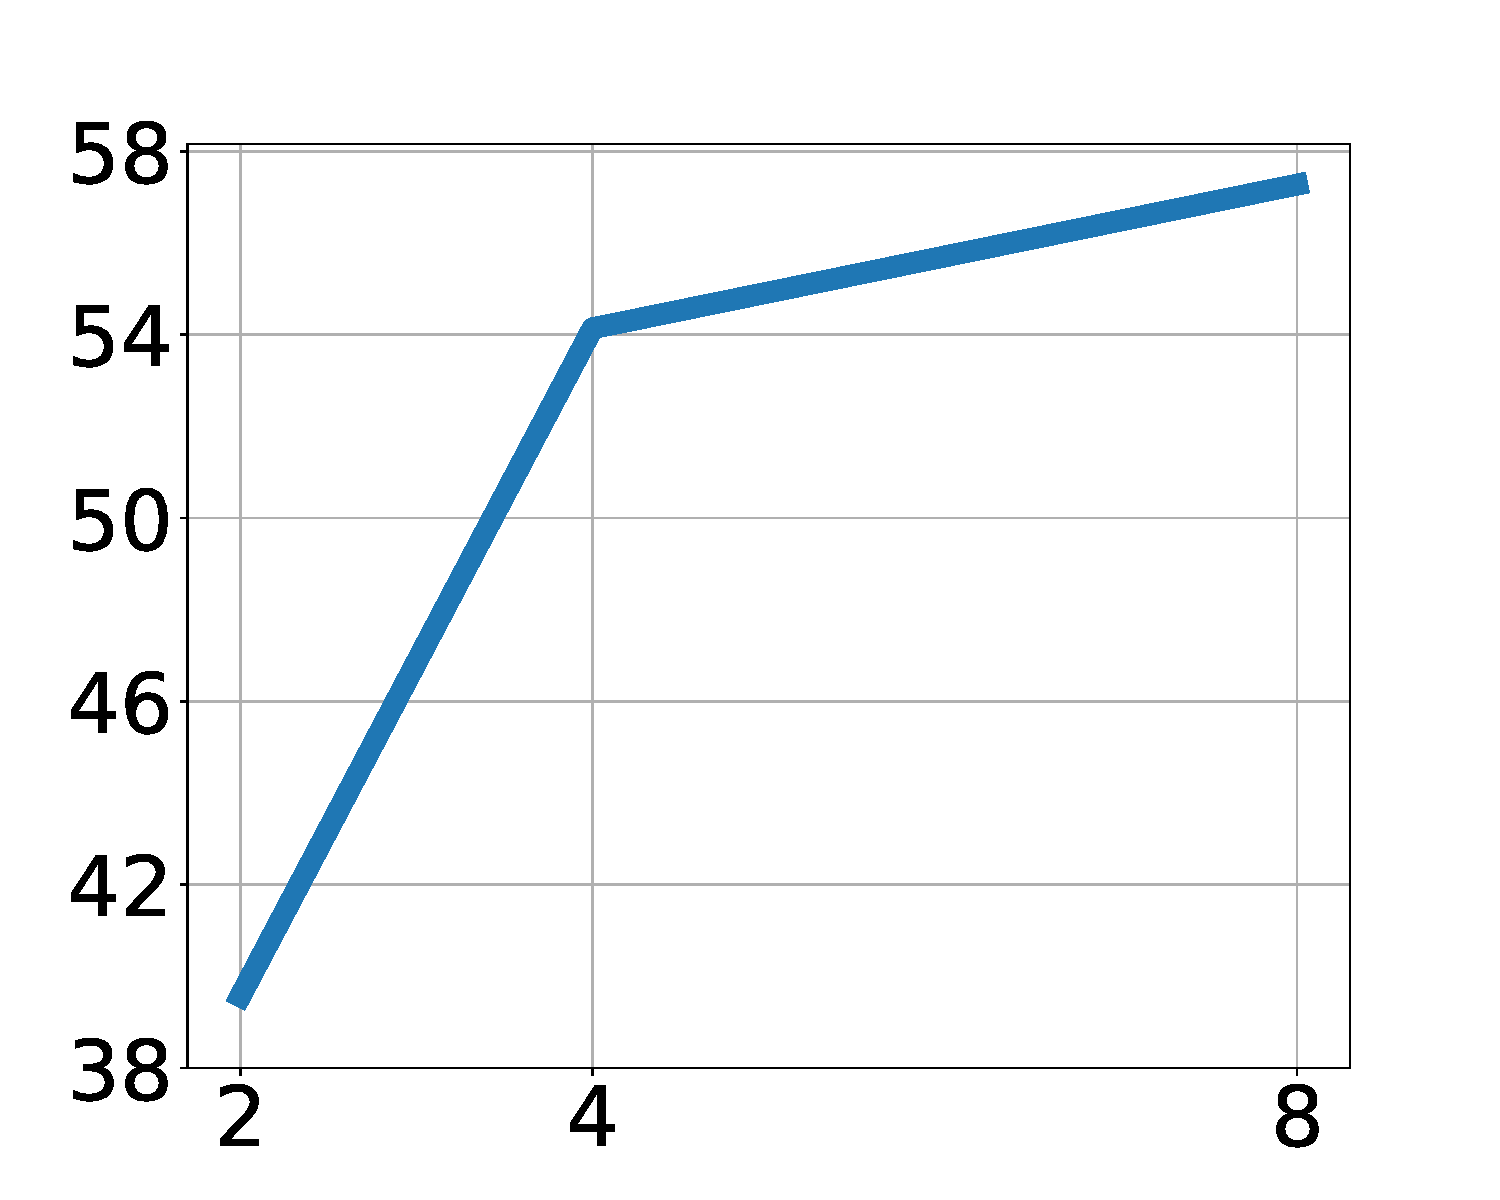
\includegraphics[width=\linewidth]{figs/fig5d_vocab.pdf}\\{\scriptsize latent vocabulary}\end{minipage}
  \credit{Fig.~5: average success rate (\%)}
  {\tiny\color{mute} \S5.1 reads panel (c) as Language Table; App.~F describes Fig.~5 as
    Bridge and SIMPLER throughout. Check before quoting a single panel.\par}
\end{frame}

\begin{frame}{Backup: camera motion as a code}
  \centering
  \paperfig{width=0.9\linewidth}{figs/fig14_camera.pdf}{Fig.~14}
\end{frame}

% No allowframebreaks: with it, multicols emits a blank page and clips the last entry.
\begin{frame}[t]{References}
  \vspace{-1.2em}
  \nocite{ye2025lapa}
  {\tiny\linespread{0.84}\selectfont
  \setlength{\bibsep}{0.2pt plus 0.2pt}
  \setlength{\columnsep}{1em}
  \begin{multicols}{2}\bibliography{refs}\end{multicols}}
\end{frame}

\end{document}
